\documentclass[11pt]{article}
\usepackage[a4paper, margin=1in]{geometry}
\usepackage{amsmath, amssymb}
\usepackage{hyperref}
\usepackage{graphicx}
\usepackage{titlesec}
\usepackage{listings} 
\usepackage{xcolor}   
\usepackage[utf8]{inputenc}
\usepackage{tikz}
\usetikzlibrary{arrows.meta, positioning, shapes.geometric}

\title{Lecture notes}
\author{}
\date{}

\titleformat{\section}{\large\bfseries}{\thesection}{1em}{}
\titleformat{\subsection}{\normalsize\bfseries}{\thesubsection}{1em}{}

\begin{document}

\setlength{\parindent}{0pt}
\setlength{\parskip}{1ex}

\maketitle

\tableofcontents

\newpage

\section{Introducción}
\subsection{Motivación}
La inferencia sin verosimilitud (\textit{likelihood-free inference}) permite estimar parámetros cosmológicos sin asumir una forma analítica para la función de verosimilitud, evitando así sesgos por supuestos incorrectos como Gaussianidad. Esto es especialmente relevante en cosmología, donde procesos no lineales y efectos sistemáticos complican el modelado estadístico. En el contexto del CMB, aunque las fluctuaciones primordiales son aproximadamente Gaussianas, efectos secundarios, como lentes gravitacionales, polarización inducida y \textit{foregrounds} introducen no-Gaussianidades que desafían los análisis tradicionales basados en espectros de potencia.

El CMB es uno de los observables más poderosos para estudiar los parámetros cosmológicos, pero su buena explotación requiere ir más allá de las estadísticas de dos puntos. En este trabajo, comenzaré con el análisis de estadísticas resumidas tradicionales, partiendo de los \textit{angular power spectrum} (APS) de temperatura, que capturan la información gaussiana primordial. Posteriormente, escalaré hacia estadísticas más complejas que incluyan modos de polarización, para finalmente explorar métodos no lineales (de ser posible).

Métodos de aprendizaje profundo, como la compresión neuronal, pueden extraer información no lineal de mapas del CMB, mejorando las restricciones sobre parámetros como $\Omega_m$ o $\sigma_8$. Además, la inclusión de efectos no ideales como ruido instrumental, cortes en el cielo y \textit{foregrounds} en simulaciones realistas es importante para un análisis robusto. Esta aproximación gradual---desde espectros de potencia hasta estadísticas de alto orden---permitirá validar resultados intermedios y cuantificar ganancias al incorporar información no gaussiana.

\subsection{Inferencia Bayesiana}
El marco bayesiano permite determinar la distribución posterior de parámetros cosmológicos $\theta$ mediante la expresión 

\begin{equation}
p(\theta|x,M) = \frac{p(x|\theta,M)p(\theta|M)}{p(x|M)}
\end{equation}

donde $x$ representa los datos observacionales y $M$ el modelo cosmológico. La determinación precisa de la función de verosimilitud $p(x|\theta,M)$ presenta varios desafíos en el análisis del CMB. Aunque las fluctuaciones primordiales son aproximadamente gaussianas, efectos secundarios como las lentes gravitacionales, la contaminación por \textit{foregrounds} y las no-linearidades instrumentales introducen complejidades. Estas complicaciones se acentúan al considerar estadísticas más allá del espectro de potencia, como los estudios de no-gaussianidad primordial o los análisis de lentes gravitacionales a pequeña escala.

Los métodos tradicionales basados en supuestos gaussianos para la verosimilitud muestran limitaciones crecientes frente a la precisión de los nuevos experimentos. Particularmente, para análisis que involucran reconstrucción de lentes, estudios de no-gaussianidad o el tratamiento de regiones con máscaras complejas, la distribución exacta de los estadísticos se desvía significativamente de la aproximación gaussiana. Esta discrepancia puede llevar a estimaciones sesgadas de parámetros cosmológicos.

\subsection{\textit{Likelihood-free inference}}
La inferencia sin verosimilitud (también llamada \textit{Simulation-based inference}) busca realizar inferencia estadística en situaciones donde la función de verosimilitud es intratable o desconocida. Métodos tradicionales como el \textit{Approximate Bayesian Computation} (ABC) abordan este problema comparando directamente los datos simulados con los datos observados mediante una métrica de distancia. En este enfoque, se generan múltiples simulaciones a partir de diferentes valores del parámetro $\theta$ y se conservan aquellos para los cuales los datos simulados $x$ se parecen lo suficiente a los datos observados, según un umbral de tolerancia. Este método depende fuertemente de la elección de estadísticas resumidas y puede requerir un número muy elevado de simulaciones para obtener una aproximación razonable de la distribución posterior. La figura 1 se muestra la pipeline general utilizada para estimar posteriores con el método ABC.

\begin{figure}[htbp]
    \centering
    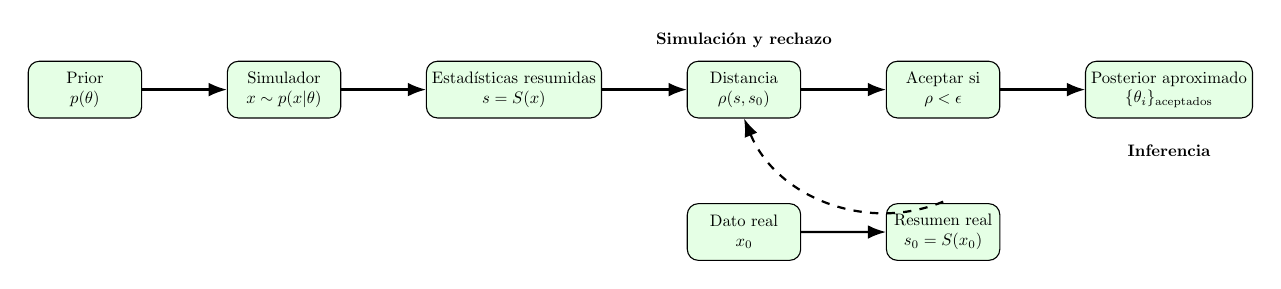
\begin{tikzpicture}[
        scale=0.6,
        every node/.style={transform shape},
        node distance=1.2cm and 1.8cm,
        box/.style={draw, rounded corners, minimum width=2.4cm, minimum height=1.2cm, align=center, fill=green!10},
        arrow/.style={-{Latex}, thick}
    ]
        \node[box] (prior) {Prior \\ \( p(\theta) \)};
        \node[box, right=of prior] (simulator) {Simulador \\ \( x \sim p(x|\theta) \)};
        \node[box, right=of simulator] (summary) {Estadísticas resumidas \\ \( s = S(x) \)};
        \node[box, right=of summary] (distance) {Distancia \\ \( \rho(s, s_0) \)};
        \node[box, right=of distance] (accept) {Aceptar si \\ \( \rho < \epsilon \)};
        \node[box, below=1.8cm of distance] (obs) {Dato real \\ \( x_0 \)};
        \node[box, right=of obs] (s_obs) {Resumen real \\ \( s_0 = S(x_0) \)};
        \node[box, right=of accept] (posterior) {Posterior aproximado \\ \( \{\theta_i\}_{\text{aceptados}} \)};

        \draw[arrow] (prior) -- (simulator);
        \draw[arrow] (simulator) -- (summary);
        \draw[arrow] (summary) -- (distance);
        \draw[arrow] (distance) -- (accept);
        \draw[arrow] (accept) -- (posterior);
        \draw[arrow] (obs) -- (s_obs);
        \draw[arrow, dashed] ([yshift=1pt] s_obs.north) to[bend left=45] (distance.south);

        \node[above=0.15cm of distance] {\textbf{Simulación y rechazo}};
        \node[below=0.45cm of posterior] {\textbf{Inferencia}};
    \end{tikzpicture}
    \caption{Pipeline general de ABC.}
    \label{fig:abc}
\end{figure}

Más recientemente, técnicas modernas basadas en aprendizaje automático han revolucionado este enfoque. En lugar de comparar datos de manera directa, estos métodos reformulan el problema como uno de estimación de densidad: se modela la distribución conjunta de pares $(\theta, x)$ simulados, lo que permite aproximar la distribución posterior $p(\theta|x)$. Herramientas como redes neuronales profundas y flujos normalizantes permiten entrenar modelos expresivos que aprenden directamente la relación entre datos y parámetros a partir de muestras sintéticas, evitando el cálculo explícito de la verosimilitud y haciendo la inferencia mucho más eficiente. La figura 2 muestra la pipeline general para técnicas de sbi basadas en aprendizaje automático.

\begin{figure}[htbp]
    \centering
    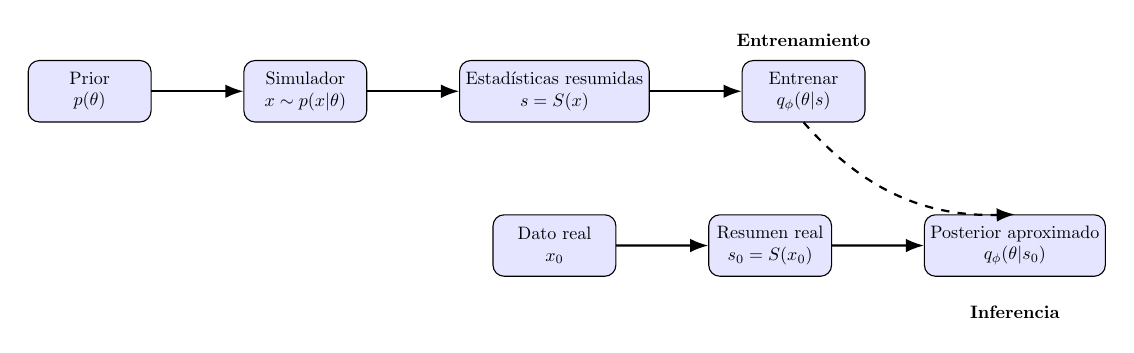
\begin{tikzpicture}[
        scale=0.65,  
        every node/.style={transform shape}, 
        node distance=1.2cm and 1.8cm,
        box/.style={draw, rounded corners, minimum width=2.4cm, minimum height=1.2cm, align=center, fill=blue!10},
        arrow/.style={-{Latex}, thick}
    ]
        \node[box] (prior) {Prior \\ \( p(\theta) \)};
        \node[box, right=of prior] (simulator) {Simulador \\ \( x \sim p(x|\theta) \)};
        \node[box, right=of simulator] (summary) {Estadísticas resumidas \\ \( s = S(x) \)};
        \node[box, right=of summary] (train) {Entrenar \\ \( q_\phi(\theta|s) \)};
        \node[box, below=1.8cm of summary] (obs) {Dato real \\ \( x_0 \)};
        \node[box, right=of obs] (s_obs) {Resumen real \\ \( s_0 = S(x_0) \)};
        \node[box, right=of s_obs] (posterior) {Posterior aproximado \\ \( q_\phi(\theta|s_0) \)};

        \draw[arrow] (prior) -- (simulator);
        \draw[arrow] (simulator) -- (summary);
        \draw[arrow] (summary) -- (train);
        \draw[arrow] (obs) -- (s_obs);
        \draw[arrow] (s_obs) -- (posterior);
        \draw[arrow, dashed] (train.south) to[bend right=25] (posterior.north);

        \node[above=0.15cm of train] {\textbf{Entrenamiento}};
        \node[below=0.45cm of posterior] {\textbf{Inferencia}};
    \end{tikzpicture}
    \caption{Pipeline general para métodos con aprendizaje automático.}
    \label{fig:sbi}
\end{figure}

El paquete \texttt{sbi}, desarrollado en Python sobre \texttt{PyTorch}, implementa este paradigma de manera flexible. Ofrece herramientas para: (1) simular datos bajo distintos parámetros $\theta$, (2) entrenar estimadores de densidad condicional $p(\theta|x)$ usando arquitecturas modernas, y (3) realizar inferencia posterior dado un conjunto de datos observados. La calidad de las simulaciones y de las estadísticas utilizadas continúa siendo muy importante, ya que el modelo entrenado sólo puede aprender lo que está presente en los datos simulados. Sin embargo, al entrenar modelos que generalizan bien, se puede reducir de forma significativa el número de simulaciones necesarias, logrando una inferencia más precisa y escalable que con métodos como ABC.

\section{Simulador}
\subsection{Generador de APS}
El generador implementa un cálculo teórico completo de las anisotropías del fondo cósmico de microondas mediante la resolución numérica de las ecuaciones de Boltzmann a través del código \texttt{CAMB}. Parte de un conjunto de parámetros cosmológicos que definen un modelo $\Lambda$CDM estándar y devuelve su \textit APS correspondiente. En la actual implementación, el cálculo se restringe al espectro de temperatura, aunque la arquitectura del código permite una extensión futura para incluir los modos de polarización. El resultado final consiste en el APS completo expresado en microkelvin, que cuantifica las fluctuaciones de temperatura en función del multipolo $\ell$. 

\subsection{Ruido instrumental y cobertura parcial del cielo}
Para generar simulaciones realistas de los APS, se consideran dos fuentes principales de ruido: el ruido instrumental del experimento y la cobertura parcial del cielo, que introduce varianza cósmica adicional. Primero, se añade el ruido instrumental a los espectros teóricos mediante un modelo basado en la resolución angular del experimento (\(\theta_{\text{fwhm}}\)) y la sensibilidad por píxel (\(\sigma_T\)). El término de ruido instrumental \(N_\ell^{\mathrm{TT}}\) que se suma al espectro de potencia teórico \(C_\ell\) es:

\begin{equation}
N_\ell^{\mathrm{TT}} = \left(\theta_{\text{fwhm}} \cdot \sigma_T \right)^2 \exp\left[ \ell (\ell + 1) \frac{\theta_{\text{fwhm}}^2}{8 \ln 2} \right],
\end{equation}

donde \(\theta_{\text{fwhm}}\) se expresa en radianes. Esta fórmula modela el suavizado del cielo debido a la resolución finita del instrumento. Posteriormente, se simula la observación del cielo parcial considerando que solo se mide una fracción \(f_{\text{sky}} < 1\) del cielo completo. Como consecuencia, el estimador observable de \(C_\ell\), denotado \(\hat{C}_\ell\), no es determinístico, sino una variable aleatoria cuya dispersión depende de \(f_{\text{sky}}\). Para multipolos bajos (\(\ell < \ell_{\text{transition}}\)), se modela esta varianza como una distribución chi-cuadrado escalada:

\begin{equation}
\hat{C}_\ell = \frac{1}{\nu_\ell} \sum_{i=1}^{\nu_\ell} X_i^2, \quad X_i \sim \mathcal{N}(0, \sqrt{C_\ell}),
\end{equation}

donde \(\nu_\ell = \text{round}(f_{\text{sky}} \cdot (2\ell + 1))\) representa el número efectivo de grados de libertad. Esta formulación captura correctamente la dispersión estadística del estimador cuando el número de modos disponibles es pequeño. Para multipolos altos (\(\ell \geq \ell_{\text{transition}}\)), se asume que el estimador puede aproximarse mediante una distribución normal centrada en \(C_\ell\) con varianza:

\begin{equation}
\hat{C}_\ell \sim \mathcal{N}\left(C_\ell, \frac{2 C_\ell^2}{f_{\text{sky}} (2\ell + 1)} \right).
\end{equation}

Este enfoque es válido debido al teorema central del límite, ya que en esta región el número de modos es suficientemente grande como para justificar una aproximación gaussiana.


\end{document}